\section{Evaluation}
\label{sec:evaluation}
To evaluate the performance of the \SystemName library, we wrote a series of benchmark tests.
Not only did we test the performance of \SystemName using proxy re-encryption, but we also compared it to an RSA implementation.
Note that actually implementing \SystemName with RSA instead of PRE would defeat the purpose, as either the proxy would have to be trusted with every instance's private key, or all instances of the same function would have to share the same key pair.

For the RSA implementation, we only benchmarked the \SystemName functions responsible for encrypting and decrypting messages, since "re-encryption" is not a concept in RSA.
For the proxy re-encryption implementation, we benchmarked the \SystemName functions responsible for encrypting and decrypting messages, generating re-encryption keys, and re-encrypting messages.
Additionally, we benchmarked the underlying proxy re-encryption functions, from the PRE library we wrote.
For example, the \texttt{samba.Encrypt} function contains the following code:
\begin{lstlisting}[language=Go]
m := pre.RandomGt()
ct1 := pre.Encrypt(pp, m, pkPRE)
key := pre.KdfGtToAes256(m)
ct := AESGCMEncrypt(key, plaintext)
\end{lstlisting}
We benchmarked all three of the PRE library functions in this code snippet, as well as the \SystemName encrypt function that calls them.
All benchmarks were run using the Go testing framework, which provides a simple way to measure the time taken by each function.

\begin{figure}
	\centering
	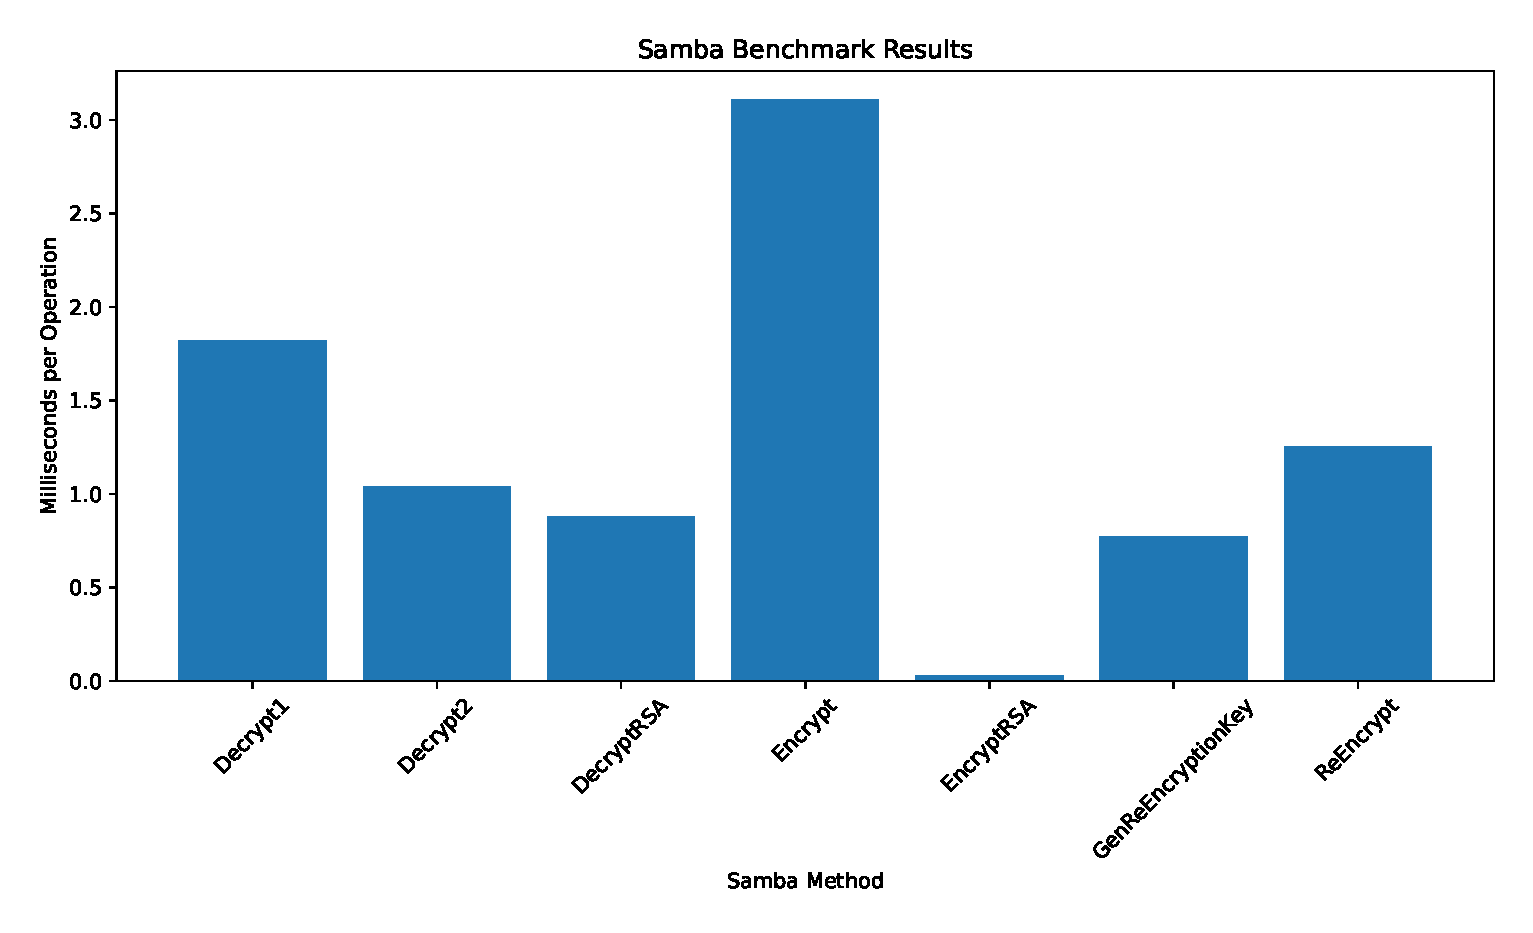
\includegraphics[width=0.48\textwidth]{figs/samba-bench}
	%
	\caption{Benchmark results for the \SystemName library, with both PRE and RSA operations.}
	%
	\label{fig:samba-bench}
\end{figure}

\begin{figure}
	\centering
	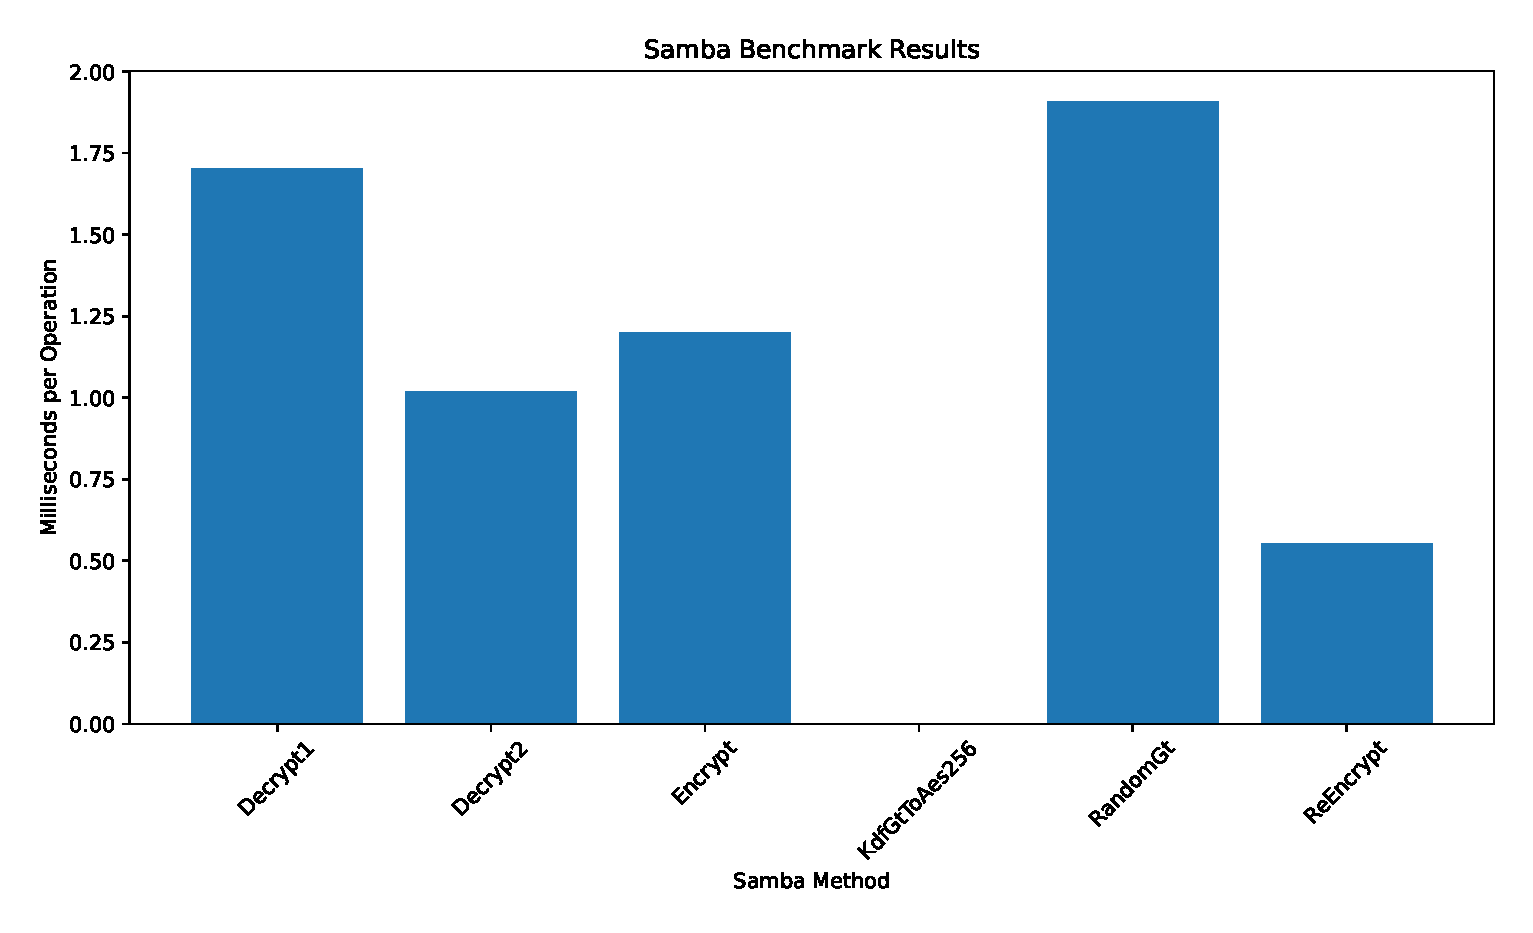
\includegraphics[width=0.48\textwidth]{figs/pre-bench}
	%
	\caption{Benchmark results for the PRE library.}
	%
	\label{fig:pre-bench}
\end{figure}


Our results from an 8-core M1 Mac of for the \SystemName benchmarks are shown in Figure~\ref{fig:samba-bench}, and the PRE benchmarks are shown in Figure~\ref{fig:pre-bench}.

The cost of RSA encryption is basically negligible, and almost invisible in Figure~\ref{fig:samba-bench}. Samba encryption, on the other hand, is our most expensive operation.
This is because it calls all three of the PRE functions mentioned above. The \texttt{pre.RandomGt} function takes about $1.9$ milliseconds, and the \texttt{pre.Encrypt} function takes about $1.2$ ms in our benchmarking.
Those two make up the bulk of the cost of \SystemName's \texttt{Encrypt}, which in total takes almost $3.2$ ms. 

RSA decryption takes much longer than RSA encryption, and both of our \SystemName decryption operations only incur slight additional overhead. The more expensive of the two, \texttt{Decrypt1}, is less than twice as expensive as RSA.

We believe the security guarantees of \SystemName justify the performance costs.
Since \SystemName is to be used exclusively in FaaS systems, network request latency, which is usually in the hundreds of milliseconds, will dominate our cryptographic slowdowns.
Additionally, the method to generate a re-encryption key doesn't have to be called on a per-request basis, but rather only the first time traffic is rerouted from the leader to an instance.
